\input{shared/ietf-slides.tex}

% about the presentation
\title{Cacheable OSCORE}
\subtitle{\texttt{draft-amsuess-core-cachable-oscore-11}}
\author{\textit{Christian~Amsüss}, Marco~Tiloca}
\date{2025-07-22, CoRE at IETF123 / Madrid}

\begin{document}

\frame{\titlepage}

\begin{frame}{Context}\Large
    \begin{itemize}
        \item CoAP: REST! Proxies!

        \item OSCORE: Proxies fragment and retransmit but do not cache.
        \item Cacheable OSCORE: … but maybe we can.
    \end{itemize}

    \vspace{1cm}

    ←: \ietfdraft{ietf-core-oscore-groupcomm} (in Last Call)

    →!: \ietfdraft{tiloca-t2trg-sw-update-groupcomm}, \ietfdraft{ietf-core-observe-multicast-notifications}\footnote{Aspirationally.}

    →?: \ietfdraft{core-dns-over-coap}, \ietfdraft{ietf-core-groupcomm-proxy}, …
\end{frame}

{
\setbeamercolor{background canvas}{bg=black}
\begin{frame}{}\Large
    \center
    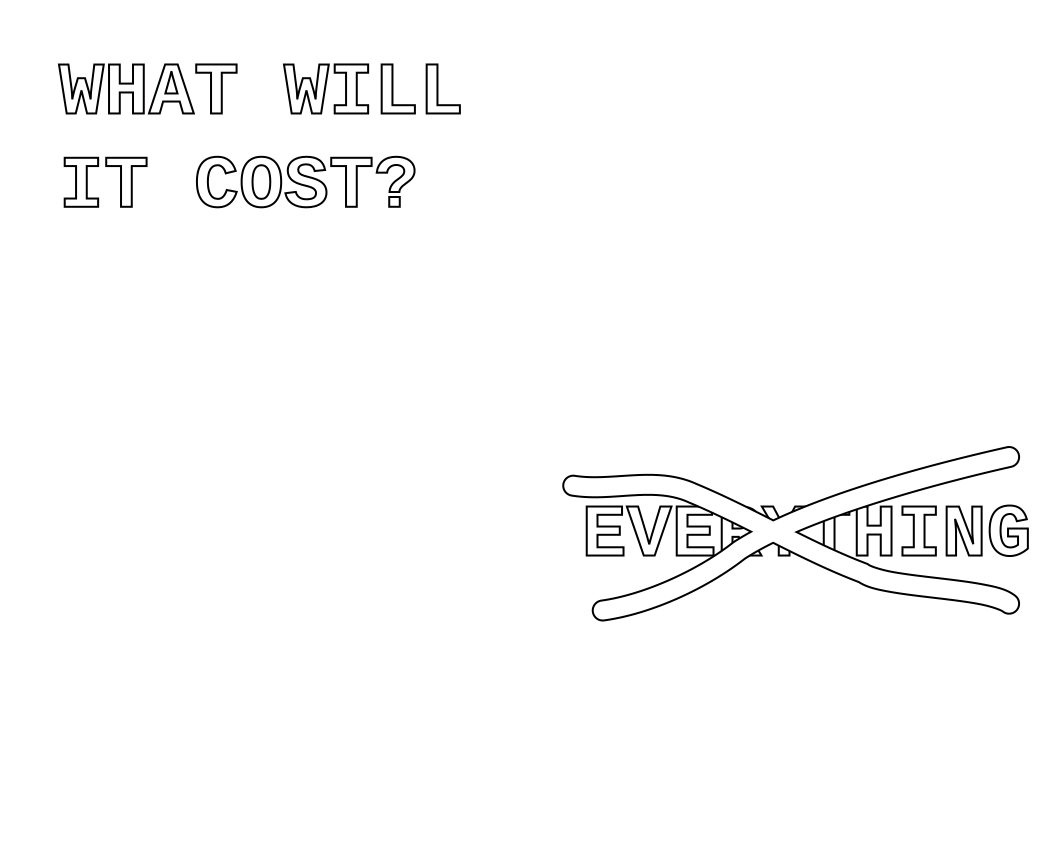
\includegraphics[width=0.6\textwidth]{cost.pdf}
\end{frame}
}

\begin{frame}{Security properties lost}\Large
    \begin{enumerate}
        \item Replay protection.
        \item Source authentication on the request.

        \item Freshness is limited. % Can still ask ETag in private.

        \item Request privacy is limited. % ietf-core-oscore-capable-proxies} help a bit.
    \end{enumerate}
\end{frame}

\begin{frame}{Document structure}\framesubtitle{Sections, as presented at IETF112}\Large
    \begin{enumerate}
        \item[2.] What happens to OSCORE when source authentication is missing?
        \item[3.] Deterministic requests:
            \begin{itemize}\Large
                \item Building requests with best-effort determinism.
                \item Initializing key material that won't suffer nonce reuse.
                \item Request-response binding as per 2.
            \end{itemize}
    \end{enumerate}
\end{frame}

\begin{frame}{Mechanics}\framesubtitle{Based on Group OSCORE}\Large
    \begin{enumerate}
        \item Establish Group OSCORE membership.
            
            {\normalsize
            GM indicates Sender ID of The Deterministic Client in extra field.
            }
        \item Prepare COSE Encrypt0 (no key yet).
        \item Hash all inputs.
        \item Derive key like pairwise, but use hash instead of ECDH output.
        \item Send pairwise-ish request.
        \item Response in group mode, request-bound by invisible Class-I option.
    \end{enumerate}
\end{frame}

\begin{frame}{What is missing?}\Large
    \begin{itemize}
        \item Which AEAD algorithms are deterministic? All current.
        \item Extra pair of eyes on security (e.\,g. on whether constant-time is needed anywhere).
        \item Does anyone need more of Section 2?
    \end{itemize}
\end{frame}

\begin{frame}{Status}\Large
    Successful interop between Californium and aiocoap implementations.
    Test vectors present.

    \bigskip

    Working Group Adoption call is still open.

    \vspace{1cm}
    
    Questions? Reviewers?
\end{frame}

\end{document}
